\documentclass[../chapter_2.tex]{subfiles}
\addbibresource{../../Thesis.bib}

\begin{document}
Once in the air, aircraft must be efficient at generating lift forces on the airframe to sustain flight. Since the early 1920's, the National Advisory Committee for Aeronautics (NACA) started tested oblique elliptical shapes in wind tunnels known as \textit{airfoils}. A wind tunnel is a machine that generates straight-line "wind" to simulate the testing object flying through the air (Figure \ref{fig:windtunnel}).

\begin{figure}[!h]
        \centering
    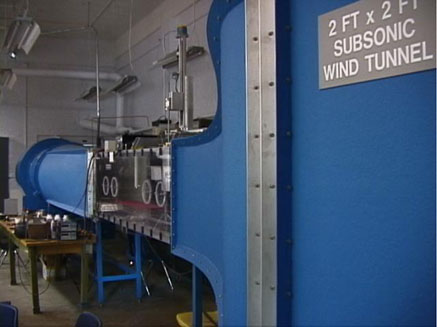
\includegraphics[width=.75\linewidth]{../../Figures/opencircuitwindtunnel.jpg}
    \caption{Subsonic wind tunnel in Auburn University's Aerodynamics Laboratory.}
    \label{fig:windtunnel}
\end{figure}

For the aircraft presented in this thesis, a \textit{Wortmann FX 63-137} is used. Figure \ref{fig:airfoil} shows the side profile.

\begin{figure}[!h]
        \centering
    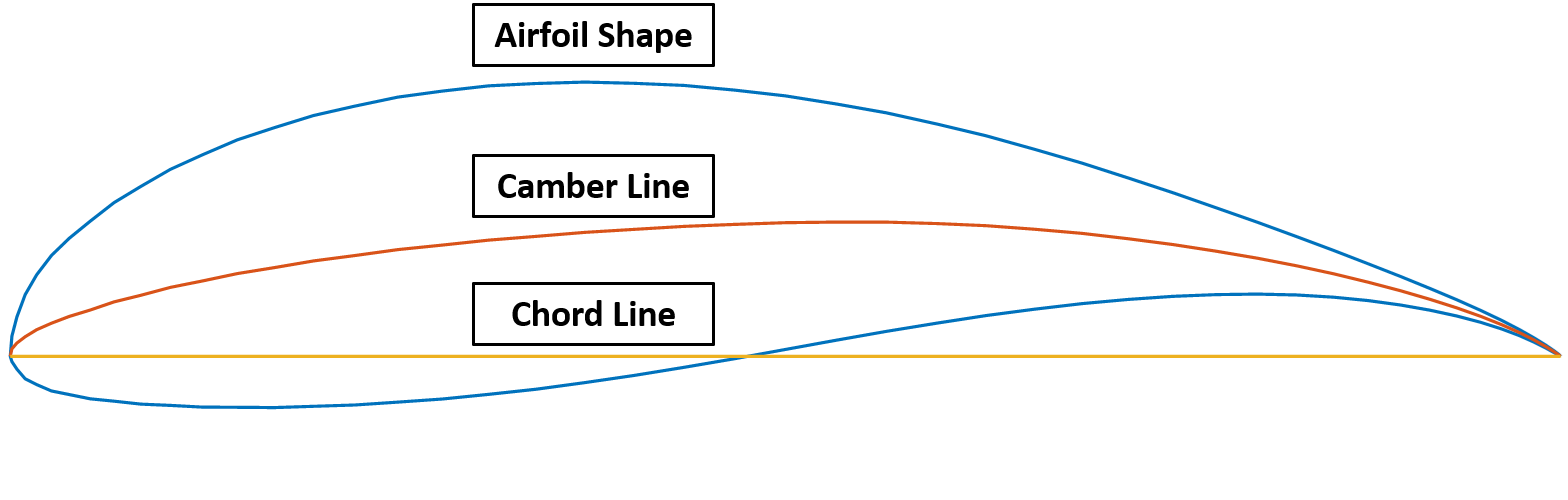
\includegraphics[width=\linewidth]{../../Figures/da40airfoil.png}
    \caption{Wortmann FX 63-137 airfoil modeled on simulated Diamond DA-40 aircraft.}
    \label{fig:airfoil}
\end{figure}
\end{document}